%%%============================================================================
%
%   Pandoc template to convert to latex using emulateapj.
%   
%
%   Usage:
%   ------
%
%   pandoc --template=[/Path/To/File/]pandoc-apj.latex
%
%
%
%   Caveats (mostly limitations in pandoc):
%   ---------------------------------------
%
%   + Doesn't do figure* and table* environments, these must be tweaked 
%     manually from standard figure and table environments or inserted as raw
%     LaTeX rather than Markdown figure invironments.
%     UPDATE: This can be accomplished by using Scholdoc rather than Pandoc.
%   + Same goes for equations: pandoc (at the time of writing) only does
%     displaymath, equations must be declared in raw LaTeX
%   + Graphics are not scaled, because the autoscale function provided in the
%     template is using the raw TeX \def function, which is not supported in
%     ApJ. UPDATE: This has been fixed in Pandoc, and Scholdoc even better.
%     Use Scholdoc! 
%
%   Copyright 2014-2016 T. E. Rivera-Thorsen.
%
%%%============================================================================
\documentclass[preprint2]{aastex6}
% \usepackage{lmodern}
% \usepackage{dcolumn}
\usepackage{amssymb,amsmath}
\usepackage[T1]{fontenc}
\usepackage[utf8x]{inputenc}
% \usepackage{natbib}
\bibliographystyle{aasjournal}
\usepackage{listings}
\usepackage{graphicx}
%\ifxetex
%  \usepackage[setpagesize=false, % page size defined by xetex
%              unicode=false, % unicode breaks when used with xetex
%              xetex]{hyperref}
%\else
%\usepackage[unicode=true]{hyperref}
%\fi
\hypersetup{breaklinks=true,
           bookmarks=true,
           pdfauthor={},
           pdftitle={Neutral ISM, Lyman-Alpha and Lyman-continuum in nearby starburst Haro 11},
           colorlinks=true,
           citecolor=blue,
           urlcolor=blue,
           linkcolor=magenta,
           pdfborder={0 0 0}}
\urlstyle{same}  % don't use monospace font for urls
% \setlength{\parindent}{0pt}
% \setlength{\parskip}{6pt plus 2pt minus 1pt}
% \setlength{\emergencystretch}{3em}  % prevent overfull lines
% \setcounter{secnumdepth}{5}

\shorttitle{Neutral ISM, Ly-Alpha and LyC in Haro 11}

\shortauthors{T. E. Rivera-Thorsen et al.}





% % \date{\today}
% 
\usepackage[caption=false]{subfig}

%%%-----------------------------------------------------------------------
%      Macros
%%%-----------------------------------------------------------------------

\begin{document}

\title{Neutral ISM, Lyman-Alpha and Lyman-continuum in nearby starburst Haro 11\footnotemark[1]}
\footnotetext[1]{Based on observations Cosmic Origins Spectrograph on the Hubble Space
Telescope, program GO 13017, PI Timothy Heckman}

\author{T. Emil Rivera-Thorsen\altaffilmark{2, 3}}

\author{Göran Östlin\altaffilmark{2, 3}}

\author{Matthew Hayes\altaffilmark{2, 3}}


\altaffiltext{2}{Department of Astronomy, Oskar Klein Centre, Stockholm University,
AlbaNova University Centre, SE-106 91 Stockholm, Sweden}
\altaffiltext{3}{Oscar Klein Centre for Cosmoparticle Physics, Department of Astronomy,
Stockholm University, Stockholm, Sweden}

\begin{abstract}
Star forming galaxies are believed to be the main source of ionizing
radiation responsible for reionizing the early Universe. Direct
observations have however been few and with escape fractions far below
what would be necessary to account for the ionization history of the
Universe. Especially in the local Universe, only a few handfuls of
emitters have been observed with typical escape fractions of a few
percent. It seems the mechanisms regulating this escape need to be ones
that are strongly evolving with redshift, if galaxies are to be held
responsible for the reionization. Gas mass, star formation feedback and
thus star formation activity are among the main suspects, known to both
regulate neutral gas coverage and evolve with cosmic time. In this
paper, we present a reanalysis of far-UV HST-COS spectra of the first
detected Lyman-continuum leaker in the local Universe, Haro 11, in which
we examine the connections between Lyman-continuum leakage and
Lyman-$\alpha$ line shape and feedback-influenced neutral ISM properties
like kinematics, geometry and column density. In particular, we discuss
the two extremes of an optically thin, density bounded ISM and a
riddled, optically thick, ionization bounded ISM and how Haro 11 fit
into the theoretical predictions made from these models. We find that
the most likely ISM model for Haro 11 knot C is one of clumpy neutral
medium with a highly ionized interclump medium with a combined covering
fraction of near-Unity and a with a residual neutral gas column density
of $XX N_{HI} < XX$, high enough to be optically thick to
Lyman-$\alpha$, but low enough to be at least partly transparent to
Lyman-continuum.
\end{abstract}

\section{Introduction and
Observations}\label{introduction-and-observations}

\subsection{Background:}\label{background}

\subsection{About Haro 11:}\label{about-haro-11}

Some of the same stuff as in Rivera-Thorsen et al. (in prep.) could be
mentioned, with a different emphasis. Star formation rate should be
mentioned from \citet{Adamo2010}. Population from same and from
\citet{Micheva2010}. Knots named by \citet{Vader1993}, and also
mentioned by \citet{Kunth2003}. It's an LBA \citep{Hoopes2007}, and an
LAE analog \citep{Hayes2007, Leitet2011}. Knot C a strong Ly$\alpha$
emitter \citep{Hayes2007}, and also a LyC leaker
{[}\citet{Bergvall2006}; Leitet2011{]}. Kinematics, it's a merger
\citep{Ostlin1999, Ostlin2001, Ostlin2015}. More weight on the
Lyman-$\alpha$ escape thing, and LyC. Mention Ly$\alpha$ escape and the
history here, too? References:

This observation is first (?) published in \citet{Alexandroff2015}, and
also in \citet{Verhamme2015} in which the Ly$\alpha$ profile is dicussed
as a .

This observation is part of the sample in \citet{Alexandroff2015}, in
which details about observation and data reduction are described in
depth; we pint the reader there for further information about these. The
Ly$\alpha$ profile in this spectrum is discussed in
\citet{Verhamme2015}. \citet{Heckman2011}, \citet{Heckman2015}.
\citet{Jaskot2013}, \citet{JaskotOey}. \citet{Bouwens2012}.

In this paper, we analyze HST-COS spectra of knot C in Haro 11. The
observations were done as part of HST program GO 13017, PI Timothy
Heckman. The spectrum has first been published by
\citet{Alexandroff2015}, a sample paper in which an attempt is made of

\section{Analysis}\label{analysis}

\subsection{Individual lines}\label{individual-lines}

Figure~\ref{fig:SingleLines} shows the individual profiles of the
transitions included in our analysis; the upper panel shows transitions
of \ion{Si}{2}, lower panel of \ion{Si}{4}. It is plainly visible that
the ionization fraction is high, with the \ion{Si}{4} curves being
considerably deeper than the low-ionized lines. Looking at the upper
panel, \ion{Si}{2} $\lambda \lambda 1304, 1526$ are somewhat shallower
than \ion{Si}{2} $\lambda 1260$. The former two lines have comparable
resonator strengths, both about a factor of 10 lower than that of
$\lambda 1260$. It is thus clear that we do not find ourselves in the
optically thin regime, in which the latter line should be
correspondingly around 10 times stronger; on the other hand, it is
possible that the two weak lines are not completely saturated. In the
lower panel, the two lines have resonator strengths within a factor of 2
of each other. They are thus at first glance consistent with a medium
that is not completely opaque, but not with an optically thin one. The
stronger absorption in \ion{Si}{4} reveals a high level of ionization of
the medium covering the central cluster.

\begin{figure}
\centering
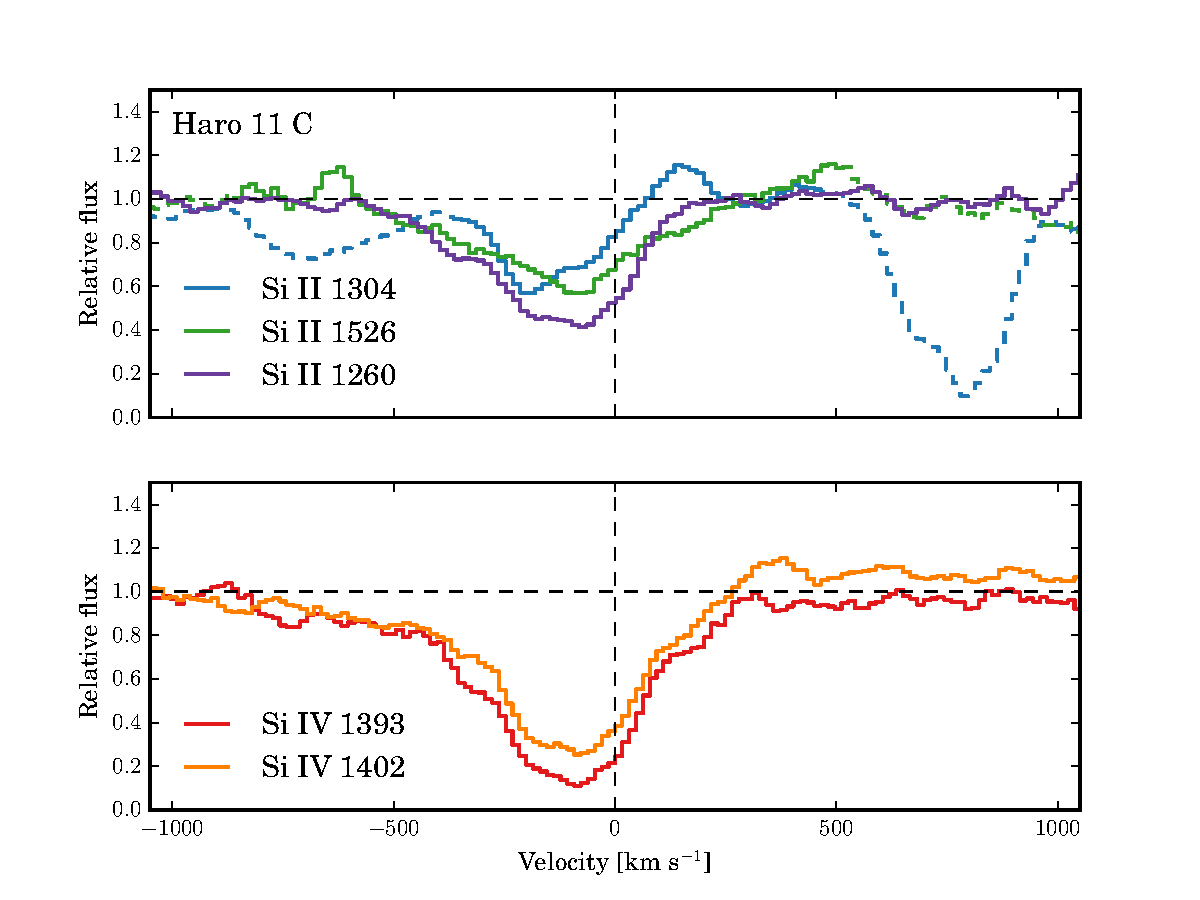
\includegraphics[width=3.500in]{../Figs/HISLISProfiles.pdf}
\caption{The \ion{Si}{2} (\textbf{upper}) and \ion{Si}{4}
(\textbf{lower}) profiles included in this
study.}\label{fig:SingleLines}
\end{figure}

\subsection{$N_{Si}$ and $f_C$}\label{sec:aod}

Following the method described in \citet{RiveraThorsen2015}; we have
performed fits for column density and covering factor in each velocity
bin, for both the high- and low-ionization state. The results are shown
in fig.~\ref{fig:WithColDens}. The upper panels show the pseudo-reduced
$\chi^2$ as defined in \citet{RiveraThorsen2015} (
$=\chi^2 / (\mathrm{DOF} + 1)$ ) for each bin, middle panels show the
inferred column density in each bin, with surrounding shaded columns
showing the confidence intervals. In the lower panels, the mean LIS line
profile is shown in black with gray shaded uncertainty intervals. On
these are overlaid the best-fit values of $f_C$ as colored dots, with
surrounding shaded bars showing the confidence intervals. We again
caution that $f_C$ is the covering fraction of HI atoms \emph{within the
given velocity bin}, and hence only provides a lower limit for the
total, geometric neutral gas covering fraction, since gas at different
velocities generally does not occupy the same projected area.

\begin{figure*}
\centering
\subfloat[LIS\label{coldenLIS}]{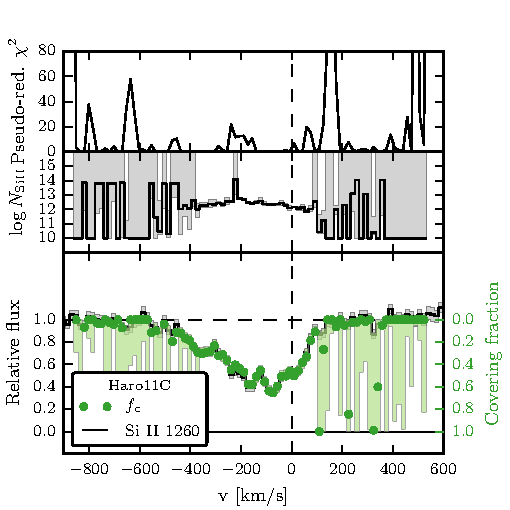
\includegraphics[width=0.400\hsize]{../Figs/Fc_haro11c_LIS.pdf}}
\subfloat[\ion{Si}{4}\label{coldenHIS}]{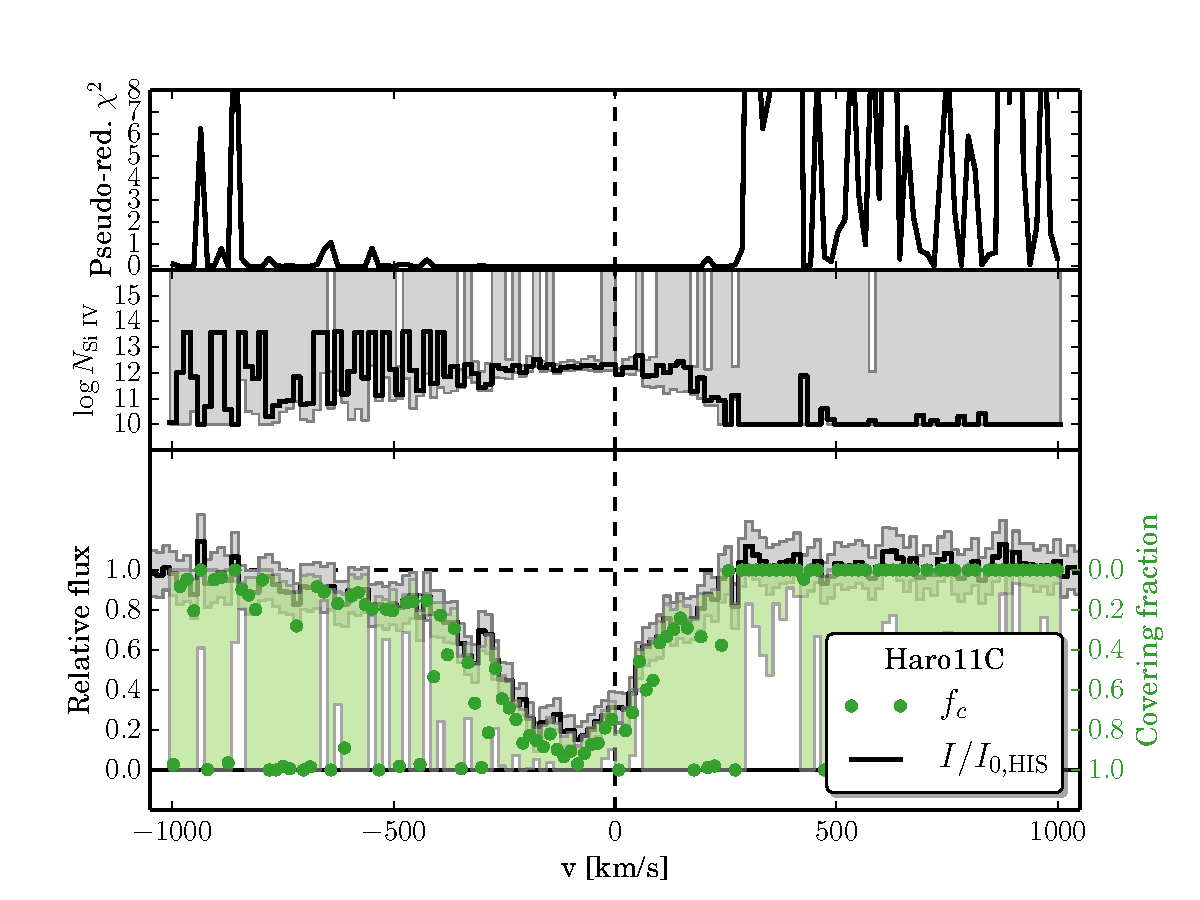
\includegraphics[width=0.400\hsize]{../Figs/Fc_haro11c-SiIV.pdf}}
\caption{\textbf{Upper panels}: Pseudo-reduced $\chi^2$ as described in
\citet{RiveraThorsen2015}. \textbf{Middle panels}: Best-fit ion column
density with confidence intervals in shaded gray. \textbf{Lower panels}:
Mean LIS/\ion{Si}{4} profile shown as black steps, with inferred $f_C$
shown with yellow dots. Lighter shaded columns show confidence intervals
for both.}\label{fig:WithColDens}
\end{figure*}

\section{Discussion and conclusions}\label{discussion-and-conclusions}

\subsection{Lyman-$\alpha$ and neutral absorption
profiles}\label{sec:LISLya}

\begin{figure}
\centering
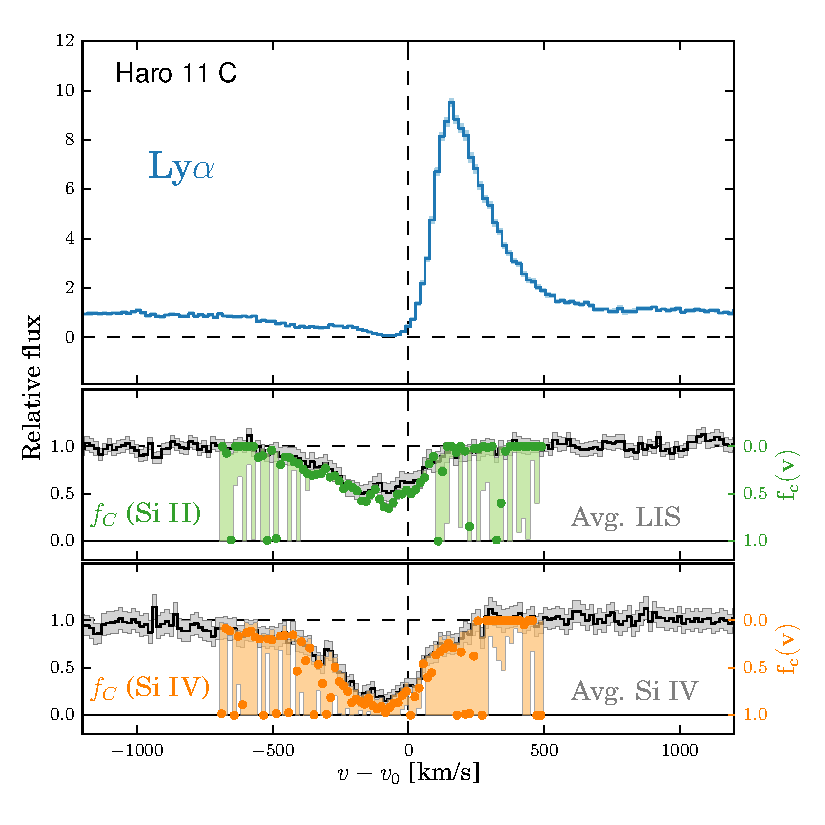
\includegraphics[width=3.500in]{../Figs/LyACoverfracs.pdf}
\caption{\textbf{Upper panel}: Ly$\alpha$ profile of Haro 11 C, in
approximate units of the surrounding continuum level. Full line is the
measured values smoothed by a 5 px. flat kernel; surrounding shading
encloses the $\pm 1 \sigma$ error band. \textbf{Middle panel}: Black
steps show the averaged, LIS line profile, smoothed by a 5px kernel.
Surrounding gray shading denotes the $\pm 1 \sigma$ confidence band.
\textbf{Lower panel}: Same as middle panel, but for the \ion{Si}{4}
transitions.}\label{fig:HisLisLya}
\end{figure}

Bla bla bla Bla bla bla

\bibliography{./main.bib}

\end{document}
